\documentclass[8pt]{beamer}

\title{Accélération Python avec GPU}
\author{Joseph Leonard Stephen Auguste}
\usetheme{Goettingen}

\usepackage[utf8]{inputenc}
\usepackage[french]{babel}
\usepackage[T1]{fontenc}
\usepackage{hyperref}
\usepackage{listings}
\usepackage{graphicx}
\usepackage{dirtytalk}
\usepackage{xcolor}
\usepackage{lstautogobble}

\addtobeamertemplate{navigation symbols}{}{%
    \usebeamerfont{footline}%
    \usebeamercolor[fg]{footline}%
    \hspace{1em}%
    \insertframenumber/\inserttotalframenumber{}
}

\definecolor{codegreen}{rgb}{0,0.6,0}
\definecolor{codegray}{rgb}{0.5,0.5,0.5}
\definecolor{codepurple}{rgb}{0.58,0,0.82}
\definecolor{backcolour}{rgb}{0.95,0.95,0.92}

\lstdefinestyle{mystyle}{
    backgroundcolor=\color{backcolour},   
    commentstyle=\color{codegreen},
    keywordstyle=\color{magenta},
    numberstyle=\tiny\color{codegray},
    stringstyle=\color{codepurple},
    basicstyle=\ttfamily\footnotesize,
    breakatwhitespace=false,         
    breaklines=true,                 
    captionpos=b,                    
    keepspaces=true,                 
    numbers=left,                    
    numbersep=5pt,                  
    showspaces=false,                
    showstringspaces=false,
    showtabs=false,                  
    tabsize=2,
    belowskip=-0.5em,
    autogobble
}

\lstset{style=mystyle}


\begin{document}

\maketitle

\section{Introduction}
\begin{frame}
    \frametitle{Qu'est-ce qu'OpenCL?}
    \say{OpenCL (Open Computing Language) est la combinaison d'une API 
    et d'un langage de programmation dérivé du C, 
    proposé comme un standard ouvert par le Khronos Group.}
    \newline
    \-- Wikipédia\pause{}
    \vspace{20pt}
    \newline
    OpenCL permet:\pause{}
    \begin{itemize}
        \item Programmer sur GPU\pause{}
        \item Parallélisation\pause{}:
            \begin{itemize}
                \item Parallélisation de tâches (task parallelism): utile si on 
                    cherche à exécuter des programmes différents en parallèle\pause{}
                \item Parallélisation de données (data parallelism): utile si on 
                    cherche à modifier différentes parties des données avec une 
                    même opération
            \end{itemize}
    \end{itemize}\pause{}
    \vspace{20pt}
    Pour l'intégrer à Python on utilise le framework \textbf{PyOpenCL}.
\end{frame}

\section{Installations}
\begin{frame}
    \frametitle{Installation d'OpenCL}
    Deux éléments sont nécessaires au fonctionnement d'OpenCL:\pause{}
    \begin{itemize}
        \item Les headers: c'est l'API qui est définie par Khronos Group\pause{}
        \item Les runtimes: c'est l'implémentation qui est définie par le 
            vendeur du GPU (Nvidia, AMD ou Intel)
    \end{itemize}
\end{frame}

\begin{frame}[fragile]
    \frametitle{Installation des headers sous Linux}
    Une ligne de commande:
    \begin{lstlisting}
       sudo apt install opencl-headers 
    \end{lstlisting}
\end{frame}


\begin{frame}[fragile]
    \frametitle{Installation des runtimes Intel sous Linux}
    Installation des \textit{compute runtime} de Intel (architecture AMD64):
    \begin{lstlisting}
    mkdir neo
    cd neo
    wget https://github.com/intel/compute-runtime/releases/download/19.14.12751/intel-gmmlib_19.1.1_amd64.deb
    wget https://github.com/intel/compute-runtime/releases/download/19.14.12751/intel-igc-core_19.11.1622_amd64.deb
    wget https://github.com/intel/compute-runtime/releases/download/19.14.12751/intel-igc-opencl_19.11.1622_amd64.deb
    wget https://github.com/intel/compute-runtime/releases/download/19.14.12751/intel-opencl_19.14.12751_amd64.deb
    wget https://github.com/intel/compute-runtime/releases/download/19.14.12751/intel-ocloc_19.14.12751_amd64.deb
    sudo apt install ./*deb
    \end{lstlisting}
    \vspace{20pt}
    \textbf{Attention:} ne pas copier coller le texte, aller chercher les 
    paquets \href{https://github.com/intel/compute-runtime/releases}{ici}.
\end{frame}

\begin{frame}[fragile]
    \frametitle{Installation des runtimes Intel sous Linux}
    L'archive à récupérer se trouve 
    \href{https://software.intel.com/content/www/us/en/develop/articles/opencl-drivers.html}{ici} 
    dans la section \say{Intel CPU Runtime for OpenCL}:
    \begin{lstlisting}[language=sh]
    tar -xvf l_opencl_p_18.1.0.015.tgz
    cd l_opencl_p_18.1.0.015/rpm
    # requires alien and libnuma1 - converts everything to deb packages
    alien *.rpm
    sudo apt install ./*deb
    # makes directories for vendors
    sudo mkdir -p /usr/lib/OpenCL/vendors/
    sudo mv /opt/intel /usr/lib/OpenCL/vendors/
    sudo cp /usr/lib/x86_64-linux-gnu/libOpenCL.so /usr/lib/OpenCL/vendors/intel/libOpenCL.so
    # configure dynamic linking
    sudo echo "/usr/lib/OpenCL/vendors/intel" > /etc/ld.so.conf.d/opencl-vendor-intel.conf
    sudo ldconfig
    \end{lstlisting}
    \vspace{20pt}
    \textbf{Attention:} les chemins ne seront pas forcément les mêmes.
\end{frame}

\begin{frame}[fragile]
    \frametitle{Installation alternative des runtimes Intel sous Linux}
    Il est possible d'installer les runtimes en une ligne de commande:
    \begin{lstlisting}[language=sh]
    apt-get install beignet beignet-dev
    \end{lstlisting}
    \vspace{20pt}
    \textbf{Attention:} Beignet n'est plus recommandé/maintenu par Intel 
    (\href{https://software.intel.com/en-us/forums/opencl/topic/758168}{source}).
    \newline
    \textbf{Non testé par moi.}
\end{frame}

\begin{frame}[fragile]
    \frametitle{Installation de PyOpenCL}
    Prérequis:
    \begin{itemize}
        \item Python installé (de préférence Python3)
        \item Pip installé (de préférence Pip3)
    \end{itemize}
    \vspace{20pt}
    Installation en une ligne de commande:
    \begin{lstlisting}[language=sh]
        pip3 install pyopencl
    \end{lstlisting}
\end{frame}

\section{OpenCL avec PyOpenCL}
\begin{frame}[fragile]
    \frametitle{Créer le contexte d'exécution}
    Pour pouvoir exécuter des programmes OpenCL dit \textbf{Kernel} 
    il faut d'abord choisir son support, créer son contexte d'exécution, 
    le compiler (build) et enfin ajouter ce contexte à la file de commandes.
    \begin{lstlisting}[language=Python]
    import pyopencl as cl
    # choose first platform 
    platform = cl.get_platforms()[0]       
    # retrive platform devices to create context
    devices = platform.get_devices()        
    # create context for platform
    context = cl.Context(devices=devices)    
    # add OpenCL source code to context (source is a string)
    program_source = cl.Program(context, source)
    # compile the kernel
    program = program_source.build()
    # enqueue the context => make the builded programs avaiable for execution
    queue = cl.CommandQueue(context)
    \end{lstlisting}
\end{frame}

\begin{frame}[fragile]
    \frametitle{Création et copies de buffers}
    Afin de pouvoir transférer des données au programme OpenCL il faut 
    commencer par définir des buffers. 
    \newline
    \textbf{Attention:} le type est très important (d'où l'utilisation de la 
    librarie numpy), il faut se référer à la documentation officielle.
    \begin{lstlisting}[language=Python]
    import numpy as np
    import pyopencl as cl
    # instantiate a numpy.ndarray of N elements of type float32 with random values
    # floats are encoded in 32bits in OpenCL
    array_in = np.random.rand(N).astype(np.float32)
    # instantiate a similar numpy.ndarray but filled with zeros
    array_out = np.zeros(N, dtype=float32)
    # context is the one created in the previous slide
    # create a read only buffer using array_in
    buffer_in = cl.Buffer(context, flags=cl.mem_flags.READ_ONLY,
                          size=array_in.nbytes)
    # create a write only buffer using array_out
    array_out = cl.Buffer(context, flags=cl.mem_flags.WRITE_ONLY,
                          size=b.nbytes)
    # copy array_in content onto GPU via buffer_in
    # is_blocking flag set to True by default
    cl.enqueue_copy(queue, src=array_in, dest=buffer_in)    
    # ... imagine execution which fills buffer_out (detailed further in the slides) ...
    # copy array_out content off GPU and onto host via buffer_out
    cl.enqueue_copy(queue, src=buffer_out, dest=array_out)
    \end{lstlisting}
\end{frame}

\begin{frame}[fragile]
    \frametitle{Exécution d'un kernel}
    L'exécution d'un Kernel se fait en appelant l'appelant sur la variable 
    \textit{program} définie précedemment.
    Disons ici que nous avons un Kernel du nom de \textit{inc} qui incrémente 
    chaque élément d'un vecteur.
    \begin{lstlisting}[language=Python]
    # ...Buffer creations and copy onto GPU....
    # Kernel function prototype: kernel void inc(global float * in, global float * out)
    kernel_arguments = (buffer_in, buffer_out)
    # run the program
    program.inc(queue,                  # aforementioned queue
                len(array_in),          # global memory
                None,                   # local memory : None if not used
                *kernel_arguments)
    # ...Copy buffer off GPU...
    \end{lstlisting}
\end{frame}

\begin{frame}[fragile]
    \frametitle{Définition du Kernel}
    Le Kernel est défini dans une chaîne de caractère 
    (peut aussi être lu d'un fichier).
    \begin{lstlisting}[language=python]
    program_source = """
        kernel void inc(global float * in, global float * out) {
            int id = get_global_id(0);
            out[id] = in[id] + 1;
        }
    """
    \end{lstlisting}
\end{frame}

\begin{frame}
    \frametitle{Notes (non négligeables)}
    Les fonctions de PyOpenCL:\@ \textit{enqueue\_copy} et du genre \textit{program.inc}
    retournent un objet de la classe pyopencl.Event. On peut appeller certaines méthodes
    sur ces objets dont notamment \textit{wait()} qui permet d'attendre la fin de 
    l'exécution de l'événement.
    \vspace{20pt}
    \newline
    L'allocation dynamique ainsi que la récursivité \textbf{n'existent pas en OpenCL.}
    De plus, seuls les tableaux dit 1D peuvent êtres passés en paramètre au Kernel.
\end{frame}

\section{Multiplication de matrices}
\begin{frame}[fragile]
    \frametitle{Kernel}
    On considère que l'on fait $a x b = c$ avec a, b et c des matrices.
    \vspace{20pt}
    \newline
    Implémentation naïve de la multiplication de matrice. Le principe est 
    qu'on itére sur les lignes et les colonnes de la matrice résultat c avec 
    les ids globaux afin de calculer la valeur d'une case de c.
    \begin{lstlisting}[language=c]
    kernel void matrix_mult(global float *a,
                            global float* b,
                            global float* c,
                            const unsigned int a_ncol,
                            const unsigned int b_ncol) {
        int rows = get_global_id(0);    /* iterate over rows */
        int columns = get_global_id(1); /* then iterate over columns */

        /* compute value */
        float value = 0;
        for (unsigned int i = 0 ; i < a_ncol ; i++) {
            value += a[rows * a_ncol + i] * b[i * b_ncol + columns];
        }

        c[rows * b_ncol + columns] = value;
    }
    \end{lstlisting} 
\end{frame}

\begin{frame}[fragile]
    \frametitle{Lancement du programme en Python}
    Afin de lancer le programme en Python on a préalablement défini des 
    tableaux pour les matrices a, b et c. On a aussi déjà défini les éléments 
    essentiels à OpenCL et compilé le Kernel.
    On obtient alors le code suivant:
    \begin{lstlisting}[language=python]
    # define buffers
    a_buffer = cl.Buffer(context, flags=cl.mem_flags.READ_ONLY, 
                         size=a.nbytes)
    b_buffer = cl.Buffer(context, flags=cl.mem_flags.READ_ONLY, 
                         size=b.nbytes)
    c_buffer = cl.Buffer(context, flags=cl.mem_flags.WRITE_ONLY, 
                         size=c.nbytes)
    # copy data into buffers
    cl.enqueue_copy(queue, src=a, dest=a_buffer)
    cl.enqueue_copy(queue, src=b, dest=b_buffer)
    # define arguments
    kernel_arguments = (a_buffer, b_buffer, c_buffer, a_nb_columns, b_nb_columns)
    # run program and wait for complemention
    program.matrix_mult(queue,
                        np.array([a_nb_rows, b_nb_columns]),
                        None,
                        *kernel_arguments).wait()
    # copy results onto host
    cl.enqueue_copy(queue, src=c_buffer, dest=c)
    \end{lstlisting} 
\end{frame}

\begin{frame}
    \frametitle{Temps de transfert des buffers}
    \begin{center}
    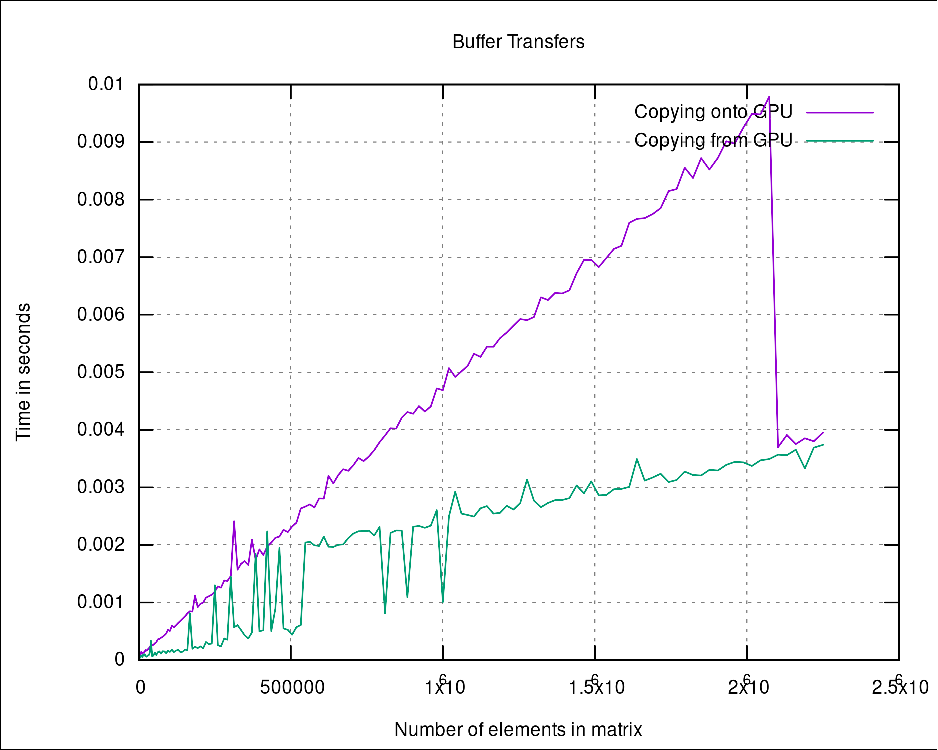
\includegraphics[width=0.9\textwidth]{../resources/matrix_naive_buffer_transfer.pdf}
    \end{center}
\end{frame}

\begin{frame}[fragile]
    \frametitle{Explication des temps de transfert des buffers}
    On voit qu'ils évoluent de façon linéaire.

    On observe cependant une augmentation en performances lorsque le nombre 
    d'éléments atteint un certain seuil pour la copie du Host au GPU:\@
    \begin{lstlisting}
    2073600	0.009790897369384766	0.003491640090942383
    2102500	0.0036971569061279297	0.0035674571990966797
    2131600	0.003909587860107422	0.003559112548828125
    2160900	0.003753185272216797	0.003653287887573242
    \end{lstlisting}
    \vspace{20pt}
    Je ne sais pas pourquoi.
\end{frame}

\begin{frame}
    \frametitle{Temps d'éxecution de la multiplication de matrices}
    \begin{center}
    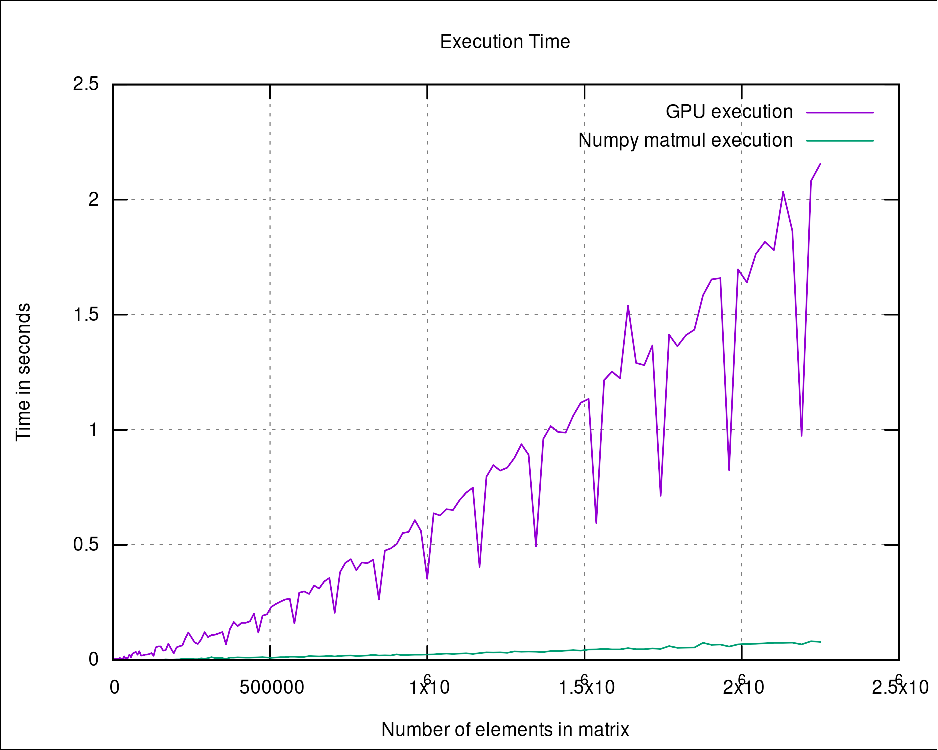
\includegraphics[width=0.9\textwidth]{../resources/matrix_naive_execution_time.pdf}
    \end{center}
\end{frame}

\begin{frame}
    \frametitle{Interprétation des temps d'éxecution}
    On observe que notre multiplication de matrice évolue rapidement 
    la complexité de l'algorithme utilisé étant $O(n^3)$.
    \vspace{20pt}
    \newline
    On observe aussi notamment que l'implémentation de Numpy est beaucoup 
    plus rapide. L'implémentation donnée est certainement sous-optimal car 
    il y a trop d'accès concurrents sur la mémoire globale.
    \vspace{20pt}
    \newline
    Enfin, on observe des piques de performances. Je ne sais pas pourquoi.
\end{frame}

\begin{frame}
    \frametitle{Précisions sur les flottants}
    \begin{center}
    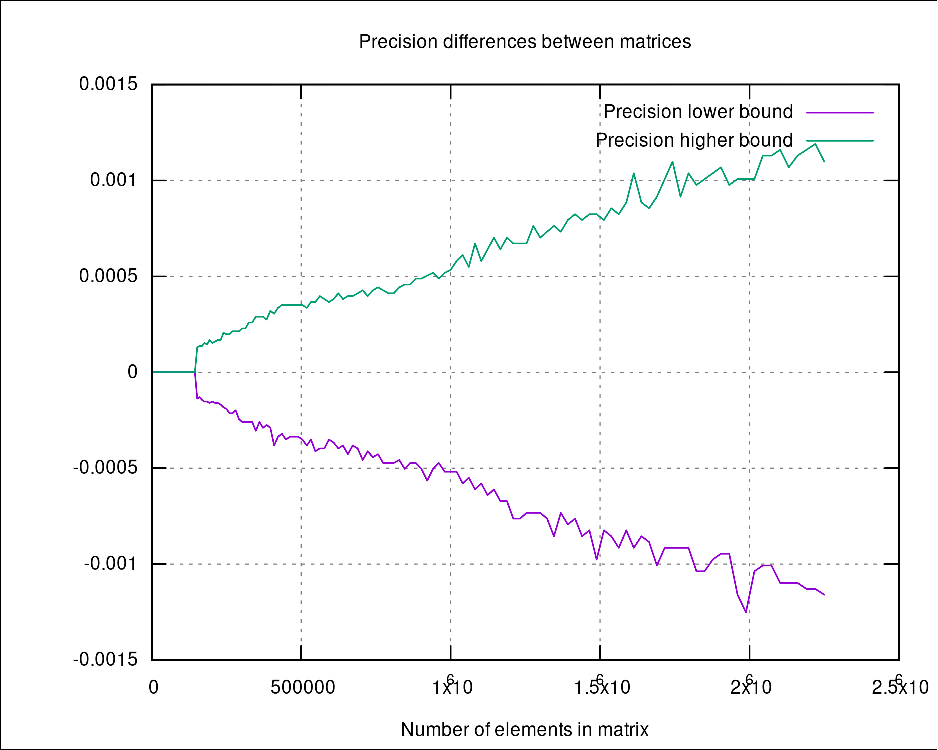
\includegraphics[width=0.9\textwidth]{../resources/matrix_naive_float_precision.pdf}
    \end{center}
\end{frame}

\begin{frame}
    \frametitle{Interprétation de la disparité des résultats}
    En comparant les résultats de Numpy.matmul et l'implémentation GPU on 
    note que plus le nombre d'éléments est grand plus l'écart existant entre 
    les résultats de l'un et de l'autre est grand. Cela s'explique par la 
    perte de précision sur les calculs de flottants. Cependant, il n'est pas 
    possible de savoir lequel des deux est le plus précis mais on se doute que 
    le GPU à des résultats plus conformes au résultats théoriques.
\end{frame}

\end{document}

%   matrix_naive_execution_time.pdf  matrix_naive_float_precision.pdf
